\section{Refinement}

The refinement relation aims at formalizing the relation between
abstract and concrete versions of the same component, or between an
abstract component and its implementation.  
In the input-enabled (or pessimistic) setting, refinement is usually
defined as trace containment or simulation
\cite{Milner71}: this ensures that the set of output behaviors of the
implementation is a subset of that of the abstract component.  
However, such definitions are not be appropriate in a
non-input-enabled setting such as our interfaces: they would also
require that the set of admissible inputs of the implementation is a
subset of that of the abstract component --- implying that the
implementation can be used in fewer environments than the abstract
component was designed for.
%
For example, if we adopted the classical definition, then the
component $\adder$ of Example~\ref{example-adder} would be refined by
a component $\strongadder$ having the same output transition relation, 
but that does not perform subtraction: precisely, with input
transition relation $\isub' = 1$. 
\mynote{fix the example, also the one on the previous section} 
%
As this example points out, refinement should be defined in a
controvariant fashion: the implementation should accept more inputs,
and produce fewer outputs, than the specification
\cite{luca-ia-01,luca-it-01}. 
This leads to the definition of refinement in terms of {\em alternating
simulation} \cite{CONCUR98AHKV}: roughly, a component $\mq$ refines
$\mp$ (written $\mq \refi \mp$) if $\mq$ can simulate all inputs of
$\mp$, and if $\mp$ can simulate all outputs of $\mq$. 

Another way to understand the need for an alternating definition of
refinement is to compare the situation for the usual models and for 
interfaces. 
The usual input-enabled (or pessimistic) models are essentially
transition systems; the natural definition of refinement for
transition systems is simulation (or trace containment). 
Interface models are essentially game models, in which the two
players, component and environment, can choose values for the
outputs and inputs, respectively; 
the appropriate definition of refinement for games is thus 
alternating simulation (or alternating trace refinement)
\cite{CONCUR98AHKV}. 
Indeed, we will see that the alternating version of refinement yields
the usual theorem about the relation between composition and
refinement (see Theorem~\ref{theo-refi}) later. 
We opt here for defining refinement in terms of alternating
simulation, rather than alternating trace containment, in order to
obtain a definition that can be checked in an algorithmically
efficient fashion \cite{CONCUR98AHKV}. 


\subsection{Refinement of Moore interfaces} 

% By encoding the refinement relation by a predicate $\rrp$, we can
% state the definition of Moore interface refinement as follows. 
% \mynote{I have a long version with the explanation as well...

Given two Moore interfaces $\mp$ and $\mq$ such that 
$\ivars_\mq \subs \ivars_\mp$ and 
$\ivars_\mp \inters (\ovars_\mp \union \ovars_\mq) = \emptyset$, 
a {\em refinement relation\/} 
$\rrel \subs \states[\vars_\mp] \times \states[\vars_\mq]$ 
from $\mp$ to $\mq$ is a relation such that, for all $(s,t) \in \rrel$:
%
\begin{itemize} 

\item If $x \in \vars_\mp \inters \vars_\mq$, 
then $s \semb{x} = t \semb{x}$.

\item For all $s_1 \in \states[\ivars_\mp]$ 
such that $(s,s_1) \sat \itrans_\mp$ 
and all $t_1 \in \states[\ovars_\mq]$ 
such that $(t,t_1) \sat \otrans_\mq$, \\
there are $s_2 \in \states[\ovars_\mp]$ 
and $t_2 \in \states[\ivars_\mq]$ \\
such that $(s,s_2) \sat \otrans_\mp$, 
$(t,t_2) \sat \itrans_\mq$, and 
$(s_1 \union s_2, t_1 \union t_2) \in \rrel$, \\
where $s_1 \union s_2$ denotes the variable assignment for $\vars_\mp$
that is the union of $s_1$ and $s_2$, and similarly for $t_1 \union t_2$. 

\item For all $s_1 \in \states[\ivars_\mp]$ 
such that $s_1 \sat \iinit_\mp$ 
and all $t_1 \in \states[\ovars_\mq]$ 
such that $t_1 \sat \oinit_\mq$, \\
there are $s_2 \in \states[\ovars_\mp]$ 
and $t_2 \in \states[\ivars_\mq]$ \\
such that $s_2 \sat \oinit_\mp$, 
$t_2 \sat \iinit_\mq$, and 
$(s_1 \union s_2, t_1 \union t_2) \in \rrel$.

\end{itemize}
%
We say that $\mq$ refines $\mp$, written $\mq \refi \mp$, if there is
a refinement relation from $\mp$ to $\mq$. 
Encoding the relation $\rrel$ by a predicate $\rrp$, we obtain the
following definition. 

\begin{defi}{(refinement of Moore interfaces)}
\label{def-moore-ref} 
Given two Moore interfaces $\mp$ and $\mq$, 
let $\avars = \ovars_\mp \setm \ovars_\mq$ be the set of ``private''
variables of the specification. 
We have that $\mq \refi \mp$ if $\ivars_\mq \subs \ivars_\mp$ and 
$\ivars_\mp \inters (\ovars_\mp \union \ovars_\mq) = \emptyset$, 
and if there is a predicate $\rrp$ on $\vars_\mp \union \vars_\mq$
such that the following formulas are valid: 
%
\begin{eqaligntwo} 
\label{eq-moore-ref} 
& \rrp \und \itrans_\mp \und \otrans_\mq \im 
  \exists (\ovars_\mp \setm \ovars_\mq)'. 
	(\itrans_\mq \und \otrans_\mp \und \rrp') & 
& \iinit_\mp \und \oinit_\mq \im \exists \avars .
	(\iinit_\mq \und \oinit_\mp \und \rrp).  \qed 
\end{eqaligntwo}
\end{defi}

\mynote{put an example here} 

\subsection{Implementation considerations} 

As is the case for normal simulation, there is a unique largest
refinement relation between two given Moore interfaces: in fact, it
can be easily seen that the union of two refinement relations is again
a refinement relation. 
Hence, in analogy to simulation, Definition~\ref{def-moore-ref}
provides an iterative algorithm for deciding refinement between
interfaces: let $\rrp_0 = \true$, and for $k \geq 0$, let 
%
\begin{equation} \label{eq-refi-comp} 
  \rrp_{k+1} = \rrp_k \und \forall (\vars_\mp \union \vars_\mq)' . 
  \bigl(\itrans_\mp \und \otrans_\mq \im 
  \exists (\ovars_\mp \setm \ovars_\mq)' . 
  (\itrans_\mq \und \otrans_\mp \und \rrp_k')\bigr).
\end{equation}
% 
Denoting with $\rrp_* = \lim_{k \go \infty} \rrp_k$ the fixpoint
(that again can be computed in a finite number of iterations), 
we have that $\mq \refi \mp$ iff 
$\iinit_\mp \und \oinit_\mq \im \exists \avars .
	(\iinit_\mq \und \oinit_\mp \und \rrp)$. 
In order to obtain an efficient implementation, we can again take
advangate for the computaton of (\ref{eq-refi-comp}) of list
representations for the transition relations, and apply
image-computation techniques. 

\mynote{complexity result?} 


\subsection{Refinement of bidirectional A/G interfaces}

Refinement of bidirectional A/G interfaces is defined similarly,
except that the refinement relation relates the locations of the two
interfaces, rather than the states. 
The definition is as follows. 

\begin{defi}{(Refinement of bidirectional A/G interfaces)}
Given two bidirectional A/G interfaces $\mp$ and $\mq$, $\mq$ refines
$\mp$ ($\mq \refi \mp$) iff there is an alternating A/G simulation
$\refi$ of $\mq$ by $\mp$ with $\hat{q}_{\mq} \refi
\hat{q}_\mp$. 

An alternating A/G simulation of $\mq$ by $\mp$ is a
binary relation $\refi \subs Q_{\mq} \times Q_\mp$ 
such that for all $(q,p) \in \refi$ we have 
(i)~$\ivars_\mq(q) \subs \ivars_\mp(q)$, 
(ii)~$\ovars_{\mq}(q) \supseteq \ovars_\mp(p)$, 
\mynote{this is different than for Moore interfaces; there I consider
any extra vars of the specification as private variables... here we
don't need this?} 
(iii)~$\phi_{\mp}(p) \im \phi_\mq(q)$, 
(iv)~$\psi_\mq(q) \im \psi_\mp(p)$, 
(v)~for all $s \in \states[\ivars_\mp]$ 
and all $t \in \states[\ovars_\mq]$, 

output valuations $o' \in [\ovars_{\mq}(q')]$ if
$\phi_\mp(q) @ i$ and $\psi_{\mq}(q') @ o'$, then $\delta_{\mq}(q',i
\uplus o') \refi \delta_\mp(q,i \uplus o')$.  \qed
\end{defi}

The notion of refinement, in addition to implementation, captures also
substitutivity: if $\mq$ refines $\mp$, and $\mp$ is compatible with
the remainder $\mr$ of the design, then also $\mr$ can be 

\begin{theo}{(substitutivity of refinement)}
\mynote{put something here} 
\end{theo}

\begin{theo}{(Substitutivity of refinements for bidirectional A/G interfaces)}
Let $F$ and $G$ be bidirectional A/G interfaces and $m$ a connection relation 
such that the composition $F \parallel_m G$ is well-formed, and let 
$F' \sqsubseteq F$. Then $F' \parallel_m G$ is well formed and 
$F' \parallel G \sqsubseteq F \parallel G$.
\end{theo}

The algorithm for composition follows directly from the definition of
composition as discussed already. We discuss here the refinement check
algorithms.

\begin{algorithm}[ht]
\caption{Refinement Check for Stateful A/G Interfaces} \label{algo1}
\begin{algorithmic}[1]
\REQUIRE two stateful A/G interfaces 
$F = (\Pi_F,Q_F,\hat{q}_F,\phi_F,\psi_F,\delta_F)$ and
$F' = (\Pi_{F'},Q_{F'},\hat{q}_{F'},\phi_{F'},\psi_{F'},\delta_{F'})$
where $\Pi_F$ stands for the stateless I/O interface $(P_F,o_F,o^+_F)$ and
$\Pi_{F'} = (P_{F'},o_{F'},o^+_{F'})$ 
\STATE Let $Prod_{F,F'} = F \circledast F' =$ a \emph{directed graph} 
$G(V_{Prod},E_{Prod})$ where 
$V_{Prod} = Q_F \times Q_{F'}$ and $E_{Prod} \subs V_{Prod} \times V_{Prod}$
such that $e = (v_1,v_2) \in E_{Prod}$ iff $v_1 = (q_1,q'_1)$, $v_2 = (q_2,q'_2)$
and $\exists$ valuations $i \in [P_F]$, $o' \in [P_{F'}]$ such that 
$\phi_F(q_1) @ i$ and $\psi_{F'}(q'_1) @ o'$ and $q_2 = \delta_F(q_1,i \uplus o')$
and $q'_2 = \delta_{F'}(q'_1,i \uplus o')$.
\STATE Let a state $v = (q,q')$ be an {\em error} state iff 
$(\Pi_{F'} \npreceq \Pi_F) \lor (\phi_F(q) \nRightarrow \phi_{F'}(q')) \lor 
(\psi_{F'}(q') \nRightarrow \psi_F(q))$, where $\preceq$ is the refinement 
relation on stateless I/O interfaces.
\IF {any error state is reachable from $(\hat{q}_F,\hat{q}_{F'})$ in 
$G(V_{Prod},E_{Prod})$}
\STATE $F'$ does not refine $F$
\ELSE
\STATE $F'$ refines $F$
\ENDIF
\end{algorithmic}
\end{algorithm}

Here is a proof that the above algorithm indeed checks refinement in stateful
A/G interfaces.

\begin{proof}{(Proof of correctness for refinement check algorithm for 
stateful A/G interfaces)}
\newline
The algorithm uses the following claim. \\
{\bf Claim:} $\hat{q}_{F'} \sqsubseteq \hat{q}_F \iff 
R(\hat{q}_{Prod},Prod_{F,F'}) \cap V_{Error} = \phi$. \\
where $V_{Error} \subs V_{Prod}$ is the set of error states and
$R(\hat{q}_{Prod},Prod_{F,F'}) \subs V_{Prod}$ is the set of vertices of 
the directed graph $G(V_{Prod},E_{Prod})$ reachable from $\hat{q}_{Prod} = 
(\hat{q}_F,\hat{q}_{F'}) \in V_{Prod}$ \\
{\bf Proof} ($\Rightarrow$) \\
We prove a stronger claim: \\
$(\hat{q}_{F'} \sqsubseteq \hat{q}_F) \Rightarrow \forall (q_F,q_{F'}) \in
R(\hat{q}_{Prod},Prod_{F,F'}), q_{F'} \sqsubseteq q_F$.
This is a stronger claim since from the definition of the refinement relation
$\sqsubseteq$, $(q_{F'} \sqsubseteq q_F) \Rightarrow (\Pi_{F'} \preceq \Pi_F
\land \phi_F(q) \Rightarrow \phi_{F'}(q')) \land (\psi_{F'}(q') \Rightarrow 
\psi_F(q))$, which means $(q_F,q_{F'}) \notin V_{Error}$.
Let $R_k(\hat{q}_{Prod},Prod_{F,F'})$ be the set of states of 
$G(V_{Prod},E_{Prod})$ which can be reached in at most $k$ steps starting 
from $(\hat{q}_F,\hat{q}_{F'})$. \\
We need to prove $\forall k \in \mathbb{N} \mathcal{P}_k$, where proposition
$\mathcal{P}_k \equiv  \forall (q_F,q_{F'}) \in 
R_k(\hat{q}_{Prod},Prod_{F,F'}), q_{F'} \sqsubseteq q_F$.
$R_0(\hat{q}_{Prod},Prod_{F,F'}) = (\hat{q}_F,\hat{q}_{F'})$.
By assumption, $(\hat{q}_{F'} \sqsubseteq \hat{q}_F)$.
Thus, $\mathcal{P}_0$ is true. \\
{\bf Inductive Step:} $\mathcal{P}_k \Rightarrow \mathcal{P}_{k+1}$ \\
Let us assume $\mathcal{P}_k \land \lnot \mathcal{P}_{k+1}$
Thus, there must be a path of length $k+1$, $(\hat{q}_F,\hat{q}'_{F'}) = 
(q_0,q'_0), (q_1,q'_1), \dots ,(q_k,q'_k), (q_{k+1},q'_{k+1})$ such that 
$\forall i = 0,1, \dots,k. q'_i \sqsubseteq q_i $, but $\lnot (q'_{k+1} 
\sqsubseteq q_{k+1})$.
For the above path to exist, there must be an edge $(q_k,q'_k) \rightarrow 
(q_{k+1},q'_{k+1}) \in E_{Prod}$. Thus there must be valuations $i \in 
[P_F]$, $o' \in [P_{F'}]$ such that $\phi_F(q_k) @ i$ and 
$\psi_{F'}(q'_k) @ o'$ and $q_{k+1} = \delta_F(q_k,i \uplus o')$
and $q'_{k+1} = \delta_{F'}(q'_k,i \uplus o')$.
However, from the definition of the refinement relation $\sqsubseteq$ we
have $q_k \sqsubseteq q'_k \Rightarrow \forall$ input valuations 
$i \in [P_F]$ and all output valuations $o' \in [P_{F'}]$ if 
$\phi_F(q_k) @ i$ and $\psi_{F'}(q'_k) @ o'$, then 
$\delta_{F'}(q',i \uplus o') \sqsubseteq \delta_F(q,i \uplus o')$.
Since this requirement is violated, we conclude $\lnot (q_k \sqsubseteq 
q'_k)$, which is a violation of our induction hypothesis.
Thus, we have reached a contradiction.
Hence we conclude that $\mathcal{P}_k \Rightarrow \mathcal{P}_{k+1}$.
The required result follows. $\square$ \\ \\
{\bf Proof} ($\Leftarrow$) \\
We define a {\em k-step alternating A/G simulation} relation 
$\sqsubseteq_k \subs Q_F \times Q_{F'}$ as follows: \\
\begin{itemize}
\item $\forall q_F \in Q_F, q_{F'} \in Q_{F'}$, $q_{F'} \sqsubseteq_0 q_F$
iff (1)$\Pi_{F'} \preceq \Pi_F$, (2) $\phi_F(q_F) \Rightarrow 
\phi_{F'}(q'_{F'}))$ and (3) $\psi_{F'}(q'_{F'}) \Rightarrow \psi_F(q_F))$
\item $\forall q_F \in Q_F, q_{F'} \in Q_{F'}$, $q_{F'} \sqsubseteq_{k+1}
q_F$ iff (1) $\Pi_{F'} \preceq \Pi_F$, (2) $\phi_F(q_F) \Rightarrow 
\phi_{F'}(q'_{F'}))$, (3) $\psi_{F'}(q'_{F'}) \Rightarrow \psi_F(q_F))$,
and (4) $\forall i \in [P_F], o' \in [P_{F'}] (\phi_F @ i \land 
\psi_{F'} @ o') \Rightarrow \delta_{F'}(q_{F'},i,o') \sqsubseteq_k 
\delta_F(q_F,i,o')$.
\end{itemize}
We present the following claim without proof: \\
{\bf Claim:} Since interfaces $F$ and $F'$ are both finite state structures,
$\hat{q}_{F'} \sqsubseteq \hat{q}_F \iff \forall k \in \mathbb{N} 
\hat{q}_{F'} \sqsubseteq_k \hat{q}_F$.
By assumption $R(\hat{q}_{Prod},Prod_{F,F'}) \cap V_{Error} = \phi$, and hence
$\hat{q}_{F'} \sqsubseteq_0 \hat{q}_F$. \\
{\bf Induction Step:} Let $\hat{q}_{F'} \sqsubseteq_k \hat{q}_F$. 
Let us assume that $\lnot (\hat{q}_{F'} \sqsubseteq_{k+1} \hat{q}_F)$.
From the definition of $\sqsubseteq_k$ it follows that this is possible
iff $\exists q_F \in Q_F, q_{F'} \in Q_{F'}$ such that $\exists i \in 
[P_F], o' \in [P_{F'}] (\phi_F @ i \land \psi_{F'} @ o'). q_{F'} = 
\delta_{F'}(\hat{q}_{F'},i,o'), q_F = \delta_F(\hat{q}_F,i,o')$, and
$\lnot ( q_{F'} \sqsubseteq_k q_F)$. It is important to note that 
the above condition implies that  the edge $(\hat{q}_F,\hat{q}_{F'}) 
\rightarrow (q_F,q_{F'}) \in E_{Prod}$.
This in turn is possible iff $\exists i \in [P_F], o' \in [P_{F'}] 
(\phi_F @ i \land \psi_{F'} @ o'). \lnot (\delta_{F'}(q_{F'},i,o') 
\sqsubseteq_{k-1} \delta_F(q_F,i,o'))$. Note that vertex 
$(\delta_F(q_F,i,o'), \delta_{F'}(q_{F'},i,o')$ is reachable from
$(\hat{q}_F,\hat{q}_{F'})$ for the same reason as before.
It is easy to see that this leads to finally $\exists q_F \in Q_F, 
q_{F'} \in Q_{F'}. \lnot(q_{F'} \sqsubseteq_0 q_F)$ and $(q_F,q_{F'})$
is reachable from $(\hat{q}_F,\hat{q}_{F'})$ in $G$.
Thus $\exists q_F \in Q_F, q_{F'} \in Q_{F'}$ such that (1) $\Pi_{F'} 
\npreceq \Pi_F$, or (2) $\phi_F(q_F) \nRightarrow \phi_{F'}(q'_{F'}))$ 
or (3) $\psi_{F'}(q'_{F'}) \nRightarrow \psi_F(q_F))$.
This directly implies that a state $q \in V_{Error}$ is reachable 
from $(\hat{q}_F,\hat{q}_{F'})$, thus $R(\hat{q}_{Prod},Prod_{F,F'}) 
\cap V_{Error} \neq \phi$, violating our initial assumption. This
contradiction proves that $\hat{q}_{F'} \sqsubseteq_k \hat{q}_F 
\Rightarrow \hat{q}_{F'} \sqsubseteq_{k+1} \hat{q}_F$. The required 
result follows. $\square$

We used the following claim in the above proof: \\
{\bf Claim:} Since interfaces $F$ and $F'$ are both finite state structures,
$\hat{q}_{F'} \sqsubseteq \hat{q}_F \iff \forall k \in \mathbb{N} 
\hat{q}_{F'} \sqsubseteq_k \hat{q}_F$.
{\bf Proof of Claim:} Let us consider the tree structure in which the root
$v_0$ is a relation $\rho_0$ given by the set ${(q_F,q_{F'}):q_F \in Q_F, 
q_{F'} \in Q_{F'}, and q_{F'} \sqsubseteq_0 q_F}$, and any other node 
$v_{k+1}$ with parent $v_k$ in the tree is the relation $\rho_{k+1}
\subs \rho_k$ such that $(q_F,q_{F'}) \in \rho_{k+1}$ iff $q_{F'} 
\sqsubseteq_{k+1} q_F$. Clearly, since both $F$ and $F'$ are finite state
structures, they must both be finitely branching and hence so must be the 
tree we have just created. Also, since $\forall k \in \mathbb{N} 
\hat{q}_{F'} \sqsubseteq_k \hat{q}_F$, this tree must be infinite. Thus 
by Koenig's Lemma, it must have at least one infinite path, and the pair
$(\hat{q}_F, \hat{q}_{F'})$ being in each relation on the path, the required 
result follows. $\square$
\end{proof}

A simple modification of the above algorithm is possible to check 
refinement in bidirectional A/G interfaces. We present the modified 
algorithm for bidirectional interfaces below, modifying the
(local) definition of an {\em error} state to take care of the
bidirectionality of ports and the state-dependence of the stateless 
I/O interface. 

\begin{algorithm}[ht]
\caption{Refinement Check for Stateful Bidirectional A/G Interfaces} \label{algo2}
\begin{algorithmic}[1]
\REQUIRE two stateful bidirectional A/G interfaces 
$F = (P_F,Q_F,\hat{q}_F,o_F,o^+_F,\phi_F,\psi_F,\delta_F)$ and
$F' = (P_{F'},Q_{F'},\hat{q}_{F'},o_{F'},o^+_{F'},\phi_{F'},\psi_{F'},\delta_{F'})$
\STATE Let $Prod_{F,F'} = F \circledast F' =$ a \emph{directed graph} 
$G(V_{Prod},E_{Prod})$ where 
$V_{Prod} = Q_F \times Q_{F'}$ and $E_{Prod} \subs V_{Prod} \times V_{Prod}$
such that $e = (v_1,v_2) \in E_{Prod}$ iff $v_1 = (q_1,q'_1)$, $v_2 = (q_2,q'_2)$
and $\exists$ valuations $i \in [P_F - o^+_F(q_1)]$, $o' \in [o_{F'}(q'_1]$ such that 
$\phi_F(q_1) @ i$ and $\psi_{F'}(q'_1) @ o'$ and $q_2 = \delta_F(q_1,i \uplus o')$
and $q'_2 = \delta_{F'}(q'_1,i \uplus o')$.
\STATE Let a state $v = (q,q')$ be an {\em error} state iff 
$(o_{F'}(q') \nsupseteq o_F(q)) \lor (o^+_{F'}(q') \nsubseteq o^+_F(q)) 
\lor (P_{F'} - o^+_{F'}(q') \nsubseteq P_F - o^+_F(q)) \lor 
(\phi_F(q) \nRightarrow \phi_{F'}(q')) \lor 
(\psi_{F'}(q') \nRightarrow \psi_F(q))$.
\IF {any error state is reachable from $(\hat{q}_F,\hat{q}_{F'})$ in 
$G(V_{Prod},E_{Prod})$}
\STATE $F'$ does not refine $F$
\ELSE
\STATE $F'$ refines $F$
\ENDIF
\end{algorithmic}
\end{algorithm}

\begin{examp}{(The Token Ring Protocol)}
The IEEE 802.5 (Token Ring) is a well-known and widely used deterministic 
LAN protocol. Figure~\ref{tokenringstate} shows an interface describing a 
IEEE 802.5-compliant node. This interface represents a node starting with
no tokens. The same diagram, with the initial state changed to $T$ would 
represent a token ring node with the token. We call these two interfaces
$NT$ and $T$ interfaces respectively.

Figure~\ref{tokenringstr} shows the structural diagram of token ring
components in a particular network configuration. The diagram shows three
nodes, communicating by means of the shared $req$ and $give$ signals. The
$req$ signal flows clockwise, and the $give$ (and hence the token) 
counterclockwise. The network is intialised with all but one node in 
state $NT$, and the sole node in state $T$ starts with the token. As long
as its $req$ input is deasserted, it continues to hold the token. When 
the token is requested, it goes into state $G$, where it may or may not 
give the token to the requesting node immediately. When it decides to 
give up the token, it asserts its $give$ output, sending the requesting 
node into state $RR$ and itself going into state $RG$. When the 
requesting node has got the token, it deasserts its $req$ output, going 
into state $T$, and this makes the other go into state $NT$, from which
the sequence continues as before. The states $RG$ and $RR$ are of
technical importance only, to ensure that the token is not lost in transit.

One would expect this protocol to fail if more than one node has the token 
simultaneously. We verify this using interface compatibility checking.
One would expect the protocol to work independent of the number of nodes
in the network. We verify this using interface refinement.

\begin{figure}[htb]
\centering
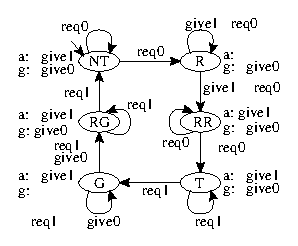
\includegraphics[scale=0.5]{tokenringstate.pstex}
\caption{Token Ring NT interface} \label{tokenringstate}
\end{figure}

\begin{figure}[htb]
\centering
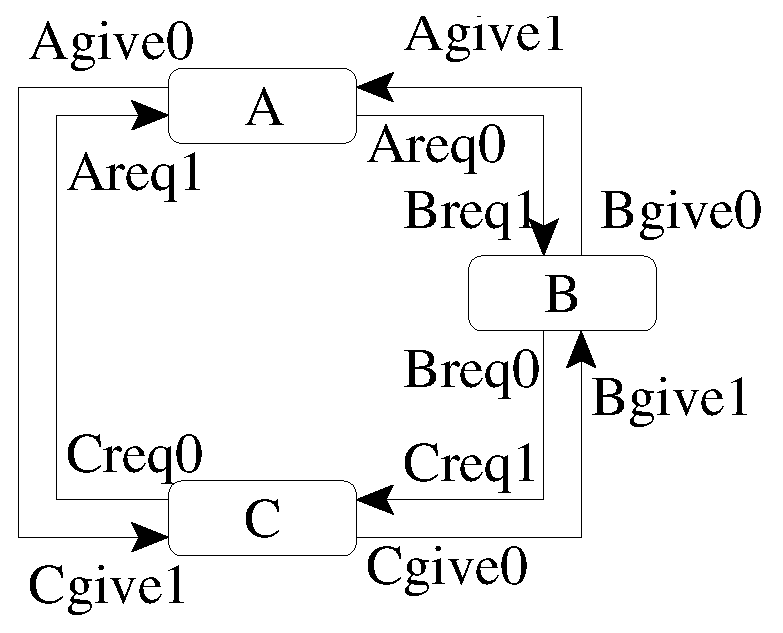
\includegraphics[scale=0.5]{tokenringstr.pstex}
\caption{Token Ring network} \label{tokenringstr}
\end{figure}

The composition of two $T$ interfaces is found to be null. Thus our tool 
verifies that two $T$ nodes are incompatible, as expected.

It verifies that a network configuration with $1$ $T$ node and any number 
of $NT$ nodes is a refinement of a network configuration with just 
$1$ $T$ node, as expected.  
Similarly a network configuration with any number of $NT$ nodes is
verified to be a refinement of a network configuration with just
one $NT$ node.

This confirms the independence of the token ring protocol of the number
of participating nodes. $\square$
\end{examp}
